%\documentclass[10pt, twocolumn]{article}
%\documentclass[11pt]{article}
%\documentclass[twocolumn,showpacs,preprintnumbers,amsmath,amssymb,prl, superscriptaddress]{revtex4}
%\documentclass[twocolumn, preprintnumbers,amsmath,amssymb,prd, superscriptaddress]{revtex4}
\documentclass[preprintnumbers,amsmath,amssymb,prd,superscriptaddress]{revtex4}
%\documentclass[10pt, preprint,showpacs,preprintnumbers,amsmath,amssymb, superscriptaddress]{revtex4}
%\documentclass[11pt, prd,preprintnumbers,amsmath,amssymb, superscriptaddress]{revtex4}
%\documentclass[11pt, prd,preprintnumbers, amsmath,amssymb, superscriptaddress, nofootinbib, hyperref]{revtex4}

\usepackage{latexsym}
\usepackage{amssymb}
\usepackage{epsfig,amsmath,graphics}
\usepackage{epstopdf}
\usepackage{verbatim}
\usepackage{wasysym}
\usepackage{hyperref}
\usepackage{feynmp-auto} % feynman diagrams
%\usepackage{subfig}
\usepackage[utf8]{inputenc}
\usepackage{xpatch}
\usepackage{xcolor}
\usepackage{mathtools}
\hypersetup{
    colorlinks,
    linkcolor={red!80!black},
    citecolor={green!60!black},
    urlcolor={blue!60!black}
}
\usepackage{appendix}

\newcommand{\Ez}{\mathcal{E}_0}
\newcommand{\Eboom}{\mathcal{E}_\text{boom}}
\newcommand{\OO}{\mathcal{O}}
\newcommand{\LL}{\mathcal{L}}
\newcommand{\HH}{\mathcal{H}}
\newcommand{\TeV}{\text{TeV}}
\newcommand{\GeV}{\text{GeV}}
\newcommand{\MeV}{\text{MeV}}
\newcommand{\keV}{\text{keV}}
\newcommand{\rad}{\text{rad}}
\newcommand{\cm}{\text{cm}}
\newcommand{\angstrom}{\buildrel _{\circ} \over {\mathrm{A}}}
\newcommand{\pslash}{p\hspace{-0.070in}/\,}
\newcommand{\Mpl}{M_{\text{pl}}}
\newcommand{\ket}[1]{\ensuremath{\left|#1\right>}}
\newcommand{\bra}[1]{\ensuremath{\left<#1\right|}}
\newcommand{\braket}[2]{\ensuremath{\left<#1|#2\right>}}
%Large Parentheses
\def\r{\right)}
\def\l{\left(}

\begin{document}

%\preprint{APS/123-QED}

\subsection{Transits}

\paragraph{Boom Condition.}
The energy deposited during a continuous heating event such as a DM transit is best described in terms of a linear energy transfer $(dE/dx)_\text{LET}$, the kinetic energy of SM particles produced per distance traveled by the DM.
If these products have a heating length $L_0$ then the relevant energy deposit must at minimum be taken as the energy transferred over the transit distance $L_0$.
Of course, we can always choose to consider energy deposits over a longer segment of the DM trajectory.
Importantly, as per the general condition \eqref{eq:energy_boom_condition} such a deposition is \emph{less} explosive unless $L_0$ is smaller than the trigger size $\lambda_T$.
Thus, we consider the energy deposited in a transit over the larger of these two length scales.
Assuming the energy of the DM is roughly constant over this heating event, the boom condition for transit heating is:
\begin{align}
\label{eq:transitexplosion}
  \left( \frac{d E}{d x} \right)_\text{LET} \gtrsim
  \frac{\Eboom}{\lambda_T} \cdot \text{Max}
  \left\{\frac{L_0}{\lambda_T}, 1 \right\}^2.
\end{align}

The above argument sums the individual energy deposits along the DM trajectory as though they are all deposited simultaneously.
This is possible if the DM moves sufficiently quickly so that this energy does not diffuse out of the region of interest before the DM has traversed the region.
We therefore require that the diffusion time $\tau_\text{diff} \approx 10^{-12} ~\text{s}$ across a heated region at temperature $T_f$ be larger than the DM crossing-time:
\begin{align}
  \tau_\text{diff} \sim \frac{L^2}{\alpha(T_f)} \gg
  \frac{L}{v_\text{esc}},
\label{eq:SlowDiffusion}
\end{align}
where $\alpha(T)$ is the temperature-dependent diffusivity, and the DM transits at the stellar escape velocity $v_\text{esc} \sim 10^{-2}$.
This condition is more stringent for smaller regions, so we focus on the smallest region of interest, $L = \lambda_T$.
\eqref{eq:SlowDiffusion} is then equivalent to demanding that the escape speed is greater than the conductive speed of the fusion wave front, $v_\text{cond} \sim \alpha(T_f) / \lambda_T$.
Numerical calculations of $v_\text{cond}$ are tabulated in \cite{Woosley}, and indeed condition \eqref{eq:SlowDiffusion} is satisfied for all WD densities.

\paragraph{Event Rate: Wind Scenario.}
The rate of transit events is given by the flux of DM passing through a WD
\begin{align}
  \Gamma_\text{transit} \sim
  \frac{\rho_{\chi}}{m_\chi} R_\text{WD}^2
  \l\frac{v_\text{esc}}{v_\text{halo}}\r^2 v_\text{halo},
\label{eq:TransitFluxCondition}
\end{align}
where $m_\chi$ is the DM mass, $\rho_\chi$ is the local DM density near the WD, and $R_\text{WD} \sim 10^{4} ~\text{km}$ is the WD radius.
Here $v_\text{halo} \sim 10^{-3}$ is galactic virial velocity, and the transit rate contains an $\OO(100)$ enhancement due to gravitational focusing.

\paragraph{WD Shielding.}
Runaway fusion only occurs in the degenerate WD interior where thermal expansion is suppressed as a cooling mechanism.
The outer layers of the WD, however, are composed of a non-degenerate gas and it is therefore essential that a DM candidate penetrate this layer in order to ignite a SN.
We parameterize this by a DM stopping power $(dE/dx)_\text{SP}$, the kinetic energy lost by the DM per distance traveled in the non-degenerate layer, and demand that
\begin{align}
\label{eq:CrustCondition}
  \left( \frac{d E}{d x} \right)_\text{SP} \ll
  \frac{m_\chi v^2_\text{esc}}{R_\text{envelope}},
\end{align}
where $R_\text{envelope} \approx 50 ~\text{km}$ is the width of a WD envelope \cite{KippenhahnWeigert}.
Note that the DM stopping power in the non-degenerate layer $(dE/dx)_\text{SP}$ and the linear energy transfer in the degenerate interior $(dE/dx)_\text{LET}$ are possibly controlled by different physics and may have very different numerical values.
In addition, a transit heating event satisfying condition \eqref{eq:CrustCondition} will have negligible energy loss over the parametrically smaller trigger size or heating length $L_0$, validating the boom condition \eqref{eq:transitexplosion}.

\subsection{Collisions and Decays}

\paragraph{Boom Condition.}
For a point-like DM-DM collision or DM decay event releasing particles of heating length $L_0$, ignition will occur if the total energy in SM products satisfies condition~\eqref{eq:energy_boom_condition}.
Such an event will likely result in both SM and dark sector products, so we parameterize the resulting energy in SM particles as a fraction $f_\text{SM}$ of the DM mass.
For non-relativistic DM, the DM mass is the dominant source of energy and therefore $f_\text{SM} \lesssim 1$ regardless of the interaction details.
With this parameterization, a single DM-DM collision or DM decay has a boom condition:
\begin{equation}
\label{eq:coldecay}
  m_\chi f_\text{SM}  \gtrsim \Eboom \cdot \text{max} \left \{\frac{L_0}{\lambda_T}, 1 \right \}^3.
\end{equation}
We are thus sensitive to DM masses $m_\chi \gtrsim 10^{16} ~\GeV$.

However, there is an interesting possibility if DM is captured in the WD that allows collisions of lower mass DM to ignite the star. 
Multiple DM-DM collisions in a sufficiently small region can occur rapidly enough to be counted as a single heating event.
This is similar in nature to a transit heating event, where multiple scatters across a transit length $\lambda_T$ can release an energy $\Eboom$ and satisfy \eqref{eq:transitexplosion} even if any individual scatter is not explosive by itself.   
If a single DM-DM collision is unable to ignite the star, the sum total of the energy released in many collisions can still result in a SN if
\begin{equation}
\label{eq:multcolboom}
 m_\chi f_\text{SM} \gtrsim \frac{\Eboom}{N_\text{mult}} \cdot \text{max} \left \{\frac{L_0}{\lambda_T}, 1 \right \}^3, ~~~~ N_\text{mult} \gtrsim 1,
\end{equation}
We define $N_\text{mult}$ as the number of collisions happening within a region of size $\text{max}\{\lambda_T,L_0\}^3$ (or smaller) during a diffusion time $\tau_\text{diff}$.
This necessarily depends on the DM-DM collision cross section, the DM-SM scattering cross section, and the evolution of the captured DM in the star. 
These are discussed in detail below. 

\paragraph{Event Rate: DM Wind.}

For the remainder of this section, all numerical quantities are evaluated assuming a WD lifetime $\tau_\text{WD} \sim 5 ~\text{Gyr}$ and central WD density $n_\text{ion} \sim 10^{31} ~\cm^{-3}$. 
At this density, the relevant WD parameters are approximately: 
\begin{equation}
v_\text{esc} \approx 2 \times 10^{-2}, ~~~~ R_\text{WD} \approx 4000 ~\text{km}, ~~~~ M_\text{WD} \approx 1.25 ~M_{\astrosun}.
\end{equation}
We also assume a typical WD temperature $T \sim \text{keV}$.

DM with negligible energy loss in the WD medium will traverse the star in $\sim R_\text{WD}/v_\text{esc} \approx 0.1 ~\text{s}$ and have a number density within the WD enhanced relative to the average galactic density by a factor $(v_\text{esc}/v_\text{halo}) \sim 10$.
In the wind scenario, the DM-DM collision rate inside the WD parameterized by a cross-section $\sigma_{\chi \chi}$ is:
\begin{align}
  \Gamma_\text{collision}
  \sim \l \frac{\rho_\chi}{m_\chi} \r^2 \sigma_{\chi \chi} \l \frac{v_\text{esc}}{v_\text{halo}}\r^3 v_\text{halo} R_\text{WD}^3.
  \label{eq:collisionDM}
\end{align}
Similarly the net DM decay rate inside the WD parameterized by a lifetime $\tau_\chi$ is:
\begin{align}
 \Gamma_\text{decay}
   \sim \frac{1}{\tau_\chi} \frac{\rho_{\chi}}{m_\chi} \l \frac{v_\text{esc}}{v_\text{halo}}\r R_\text{WD}^3.
  \label{eq:decayDM}
\end{align}

\paragraph{Event Rate: DM Capture.}
For the DM to be captured in a WD, it must lose energy $\sim m_\chi v^2$, where $v$ is the relative DM velocity (in the rest frame of the WD) asymptotically far away.
Properly, this DM velocity is described by a (boosted) Maxwell distribution peaked at the galactic virial velocity $v_\text{halo} \sim 10^{-3}$. 
For $v \ll v_\text{esc}$, we demand that the DM lose a fraction $(v/v_\text{esc})^2$ of its energy to eventually stop in the star. 

The physics of DM capture can be made more precise for a specific interaction.
Consider a spin-independent, elastic scattering off ions characterized by cross section $\sigma_{\chi A}$. 
Assuming $m_\chi \gg m_\text{ion}$, the typical momentum transfer in an elastic scatter is $q \sim \mu_{A} v_\text{esc} \approx 200 ~\MeV$, where $\mu_{A}$ is the reduced mass of the DM-nuclei system. 
This corresponds to an energy transfer $q^2/m_\text{ion} \sim m_\text{ion} v_\text{esc}^2 \approx 10 ~\MeV$. 
The average number of DM scatters during a full transit of the WD is simply a ratio of the mean free path to the size of the WD
\begin{equation}
N_\text{scatter} \sim n_\text{ion} \sigma_{\chi A} R_\text{WD}.
\end{equation}
If $N_\text{scatter} < 1$, then $N_\text{scatters}$ is the probability for a single scatter to occur during the transit. 
Thus, DM with initial velocities less than
\begin{equation}
\label{eq:capture}
v_\text{cap}^2 \sim v_\text{esc}^2 \l \frac{m_\text{ion}}{m_\chi} \r \text{max}\{N_\text{scatter} ,1\}.
\end{equation}
will be captured in the WD. 
A detailed calculation of the rate of DM capture \cite{Gould} shows that this rate is parametrically
\begin{equation}
\Gamma_\text{cap} \sim \Gamma_\text{transit} \cdot \text{min}\{N_\text{scatter}, 1\} \l \frac{v_\text{cap}}{v_\text{halo}} \r^2,
\end{equation}
valid if $v_\text{cap} \lesssim v_\text{halo}$. 
Otherwise, the capture rate is simply $\Gamma_\text{cap} \sim \Gamma_\text{transit}$, i.e. every transiting DM is captured. 
Evidently, the assumption that the scatters responsible for slowing the DM are not sufficient to blow up the WD \eqref{eq:transitexplosion} is a valid one for cross sections
\begin{equation}
\sigma_{\chi A} < \l \frac{\Eboom}{\lambda_T} \r \l \frac{1}{m_\text{ion} v_\text{esc}^2} \r \l \frac{1}{n_\text{ion}} \r \approx 10^{-8} ~\cm^2,
\end{equation}
Since the momentum transfer $q$ is roughly of order the inverse nuclear size, it is reasonable to expect the DM coherently scatters off all nucleons in the nucleus. 
The average per-nucleon cross section (spin-independent) is
\begin{equation}
\sigma_{\chi A} = A^2 \l \frac{\mu_{A}}{\mu_{n}}\r^2 F^2(q) \sigma_{\chi n},
\end{equation}
where $F^2(q) \approx 0.1$ is the Helm form factor, calculated based on the analytic expression in \cite{LUX thesis}. 
We can compare the cross section sufficient for capture \eqref{eq:capture} to the limits from direct detection experiments.
%In addition, the assumption that the DM mean free path is smaller than the size of the WD is valid for
%\begin{equation}
%\sigma_{\chi n} \gtrsim 10^{-43} ~\cm^2.
%\end{equation}
Currently, the most stringent bound on DM nuclear elastic scatters is from XENON 1T:
\begin{equation}
\label{eq:xenon}
\sigma^\text{Xe}_{\chi n} < 10^{-45} ~\text{cm}^2 \l \frac{m_\chi}{10^3 ~\GeV} \r.
\end{equation}

We now review the evolution of DM within the star once it has been captured. 
The DM slowly thermalizes to an average velocity
\begin{equation}
v_\text{th} \sim \sqrt{\frac{T}{m_\chi}} \approx 10^{-12} \l \frac{10^{16} ~\GeV}{m_\chi}\r^{1/2}.
\end{equation}
and sinks to the center of the star to the virial radius
\begin{align}
R_\text{th} \sim \l \frac{T}{G m_\chi \rho_\text{WD}}\r^{1/2} \approx 0.1 ~\cm \l \frac{10^{16} ~\GeV}{m_\chi}\r^{1/2} 
\end{align}
where its kinetic energy balances against the gravitational potential energy of the enclosed WD mass
Here we assume for simplicity a constant WD density $\rho_\text{WD} \sim n_\text{ion} m_\text{ion}$ within $R_\text{th}$.
Of course, the timescale for captured DM to thermalize and settle at $R_\text{th}$ depends on the nature of the DM-SM interaction.
The settle time has been explicitly calculated by \cite{Tinyakov} in the case that the DM is loses energy via elastic nuclear scatters.
In the first stage of thermalization after capture, the DM passes through the WD many times before the size of its orbit becomes fully contained within the star.
This occurs after a time
\begin{equation}
T_1 \sim \l \frac{m_\chi}{m_\text{ion}} \r^{3/2} \frac{R_\text{WD}}{v_\text{esc}} \frac{1}{N_\text{scatter}} \frac{1}{\text{max}\{N_\text{scatter}, 1\}}
\end{equation}
Note that this timescale is only relevant if the energy loss after a single transit is does not exceed $\sim m_\chi v_\text{esc}^2$:
\begin{equation}
\l \frac{m_\chi}{m_\text{ion}} \r \text{max}\{N_\text{scatter},1\} < 1. 
\end{equation}
One can show that this is the case for any cross sections which satisfy the XENON bound \eqref{eq:xenon}. 
In the next stage of thermalization, the DM completes many orbits within the star until dissipation from elastic scatters reduces the orbital size to the thermal radius.
The characteristic timescale for this is
\begin{equation}
T_2 \sim \l \frac{m_\chi}{m_\text{ion}} \r \frac{1}{n_\text{ion} \sigma_{\chi A}} \frac{1}{\sqrt{m_\text{ion}/T}}. 
\end{equation}
%If the DM rapidly loses energy in the star, we expect this time to be of order
%\begin{align}
%\label{eq:tdrift}
%  t_\text{settle} \sim \frac{R_\text{WD}}{v_\text{th}}
 % \approx 50 ~\text{yr} \l \frac{m_\chi}{10^{16} ~\GeV} \r^{1/2}. 
%\end{align}
We simply require that the settling time is shorter than the age of the WD
\begin{equation}
T_1 + T_2 < \tau_\text{WD}.
\end{equation}
The in-falling DM constitutes a number density of DM throughout the WD volume.
%\begin{equation}
%n(r) \sim \frac{\Gamma_\text{cap}}{r^2 v(r)}.
%\end{equation}
Integrating over the WD, the total annihilation rate for the in-falling DM is of order
\begin{equation}
\label{eq:infallrate}
\Gamma_\text{infall} \sim \frac{\Gamma_\text{cap}^2 \sigma_{\chi \chi}}{R_\text{th} v_\text{th}}.
\end{equation}
We can ignore the depletion of in-falling DM as long as \eqref{eq:infallrate} is less than the capture rate:
\begin{equation}
\label{eq:steadycollect}
\Gamma_\text{infall} < \Gamma_\text{cap}.
\end{equation}
For the rest of this section, we will evaluate all numerical quantities assuming efficient capture of the DM, i.e. $\Gamma_\text{cap} \sim \Gamma_\text{trans}$. 
In this case, condition \eqref{eq:steadycollect} is independent of $m_\chi$ and translates to an upper bound on the cross section $\sigma_{\chi \chi} < 10^{-13} ~\text{cm}^2$. 

After the initial off-set time, DM will be steadily collecting at the thermal radius.
Assuming \eqref{eq:steadycollect} is satisfied, the collection rate is roughly the same as the capture rate $\Gamma_\text{cap}$. 
However, the accumulated DM at $R_\text{th}$ is annihilating as well. 
Eventually, the collection and annihilation rates become comparable and there is an equilibrium number of DM particles at the thermal radius:
\begin{align}
N_\text{eq} \sim \l \frac{\Gamma_\text{cap} R_\text{th}^3}{\sigma_{\chi \chi} v_\text{th}} \r^{1/2} \approx 10^{19} \l \frac{10^{16} ~\GeV}{m_\chi} \r \l \frac{10^{-30} ~\cm^2}{\sigma_{\chi \chi}} \r^{1/2} \l \frac{\rho_\chi}{0.4 ~\GeV/\cm^3} \r^{1/2}.
\end{align}
Of course, there is no guarantee that this equilibrium state is achieved within the age of the WD. 
In that case, annihilations are subdominant and the total number of DM particles accumulated is simply
\begin{align}
N_\text{life} &\sim \Gamma_\text{cap} \tau_\text{WD} \approx 10^{29}  \l \frac{10^{16} ~\GeV}{m_\chi} \r \l \frac{\rho_\chi}{0.4 ~\GeV/\cm^3} \r
\end{align}
As expected, the total \emph{mass} of DM that the WD can possibly accumulate $\sim 10^{45} ~\GeV$ is independent of $m_\chi$. 
However, if the collected mass of DM at the thermal radius ever exceeds the WD mass within this volume, then there is the possibility of self-gravitational collapse of the DM.
The critical number of DM particles needed for collapse is given by
\begin{align}
\label{eq:Ncore}
    N_\text{crit} \sim \frac{\rho_\text{WD} R^3_\text{th}}{m_\chi} \approx 10^{12} \l \frac{10^{16} ~\GeV}{m_\chi} \r^{5/2}. \nonumber
\end{align}
This can only be achieved if the time to collect a critical mass of DM is shorter than the time for annihilations to deplete this mass sufficiently \emph{and} shorter than the WD lifetime. 
Thus the condition for a collapse is:
\begin{equation}
\label{eq:collapsecondition}
N_\text{crit} < \text{min}\{N_\text{eq}, N_\text{life}\}. 
\end{equation}
Importantly, we see that DM masses less than $\sim 10^{6} ~\GeV$ do not have enough time within the age of the WD in a DM density $\rho_\chi \sim 0.4 ~\GeV/\cm^3$ to collect a number $N_\text{crit}$ and begin a collapse. 
Also, DM masses greater than $\sim 10^{21} ~\GeV$ will collapse with just a single particle $N_\text{crit} < 1$.
At a given radius $r$, the time it takes for the DM to free-fall an $\OO(1)$ fraction of this distance is roughly
\begin{equation}
\label{eq:freefalltime}
t_\text{ff} \sim \frac{r}{v_\text{ff}}, ~~~~ v_\text{ff} \sim \sqrt{\frac{G N m_\chi}{r}}.
\end{equation}
Thus, the timescale for self-gravitational collapse at the thermal radius is independent of DM mass:
\begin{align}
\label{eq:collapsetime}
  t_\text{collapse} \sim \frac{R_\text{th}}{v_\text{th}} \approx 0.1 ~\text{s}.
\end{align}
Of course, it is possible that the DM initially remains thermalized while collapsing due to sufficiently strong DM-SM interactions. 
In the case of elastic nuclear scatters the DM loses a fraction $\sim m_\text{ion}/m_\chi$ of its energy per collision, so the DM is free-falling at the thermal radius as long as
\begin{equation}
\sigma_{\chi A} \lesssim \frac{1}{n_\text{ion} R_\text{th}} \l \frac{m_\chi}{m_\text{ion}}\r \approx 10^{-30} ~\cm^2 \l \frac{m_\chi}{10^6 ~\GeV} \r^{3/2}.
\end{equation}
It is straightforward to see that this is the case for any cross sections which satisfy the XENON bound \eqref{eq:xenon}.
Depletion of the collapsing DM mass becomes important when the timescale for collapse is of order the timescale for annihilation, which occurs at the characteristic radius
\begin{align}
R_{\chi \chi} \sim \sqrt{N_\text{crit} \sigma_{\chi \chi}} \approx 10^{-9} ~\cm  \l \frac{10^{16} ~\GeV}{m_\chi} \r^{5/4} \l \frac{\sigma_{\chi \chi}}{10^{-30} ~\cm^2} \r^{1/2}. 
\end{align}
The number (and mass) of collapsing DM is depleting by an $\OO(1)$ fraction at a distance $R_{\chi \chi}$, while below this radius the number is determined by the differential equation:
\begin{equation}
\frac{dN(r)}{dr} \sim \frac{N(r)^2}{r^3} \sigma_{\chi \chi}.
\end{equation}
This is only sensible if the DM collapses below the thermal radius (so we are justified calling the evolving DM density profile a ``collapse"):
\begin{align}
\label{eq:xicondition}
R_{\chi \chi} < R_\text{th}.
\end{align}
It turns out this will always be true if both \eqref{eq:collapsecondition} and the boom condition \eqref{eq:multcolboom}, described in detail below, are satisfied. 
It is possible that if $N(r)$ is substantially depleting below $R_{\chi \chi}$, then the collapse is halted. 

There are two potential evolutions of the captured DM: either the DM collapses or it does not. 
In the later case, either the DM has reached its equilibrium number at the thermal radius or is still continuing to accumulate, not yet having the critical mass necessary for collapse within its lifetime:
\begin{equation}
\label{eq:nocollapseann}
\text{min}\{N_\text{eq}, N_\text{life}\} < N_\text{crit}.
\end{equation}
First we see if this scenario allows for any meaningful constraints. 
Turning towards the boom condition for multiple collisions \eqref{eq:multcolboom}, the number of collisions that can be counted as a single heating event is roughly:
\begin{equation}
\label{eq:nocollapse}
N_\text{multi} \sim \l \frac{\text{min}\{N_\text{eq}, N_\text{life}\}}{R_\text{th}^3} \r^2 \sigma_{\chi \chi} v_\text{th} \text{max}\{\lambda_T,L_0\}^3 \tau_\text{diff}. 
\end{equation}
Even in the ``best-case" scenario of efficient capture $\Gamma_\text{cap} \sim \Gamma_\text{transit}$ and $L_0 \sim \lambda_T$, we find there is no parameter space $\{m_\chi, \sigma_{\chi \chi}\}$ where both \eqref{eq:nocollapseann} and \eqref{eq:multcolboom}---with $N_\text{multi}$ given by \eqref{eq:nocollapse}---are simultaneously satisfied. 

We instead turn our attention to collapsing DM, characterized by \eqref{eq:collapsecondition}. 
Of course, the number of collisions $N_\text{multi}$ that can be counted as a single heating event depends on where we examine the collapse. 
In general, this is given as an integral of the annihilation rate
\begin{equation}
\label{eq:capintegral}
N_\text{multi} \sim \int \l \frac{N}{r^3}\r^2 \sigma_{\chi \chi} \text{min}\{L_\text{heat}, r\}^3 dr, ~~~~ L_\text{heat} \equiv \text{max}\{\lambda_T, L_0\}
\end{equation}
integrating over the distance fell within a fixed time interval $\tau_\text{diff}$. 
The expectation is that there exists an optimal value of the lower radius at which $N_\text{multi}$ is maximized.
We denote this as $R_*$. 
However, even without knowing the details of this optimum choice, we can calculate \eqref{eq:capintegral} by considering the following limits. 
If the free-fall time \eqref{eq:freefalltime} at a distance of order $R_*$ is much larger than the diffusion time, the annihilation rate can be approximated as constant over a time $\tau_\text{diff}$.
If this free-fall time is instead much smaller than the diffusion time, the annihilation rate is a rapidly increasing function over the interval $\tau_\text{diff}$.
Therefore, \eqref{eq:capintegral} is approximated by the peak value of the annihilation rate (which is maximized at $R_*$) multiplied by the time spent at this peak (which is the time to free-fall $\sim R_*$).
Considering both these possibilities, the maximum value of \eqref{eq:capintegral} is of the form: 
\begin{equation}
\label{eq:nmulti}
N_\text{multi} \sim \l \frac{N}{R_*^3}\r^2  \sigma_{\chi \chi} v_\text{ff} ~\text{min}\{L_\text{heat}, R_*\}^3 ~\text{min}\left \{\tau_\text{diff}, \frac{R_*}{v_\text{ff}}\right \},
\end{equation}

The questions is: what is $R_*$?
Ultimately, the answer depends on the parameters $m_\chi$ and $\sigma_{\chi \chi}$. 
Suppose $\sigma_{\chi \chi}$ is independent of velocity or position.
In this case, the scaling is such that $N_\text{multi}$ is maximized at the smaller of the two scales $R_* \sim \text{min}\{R_{\chi \chi}, L_\text{heat}\}$. 
However, there may be some stabilizing pressure which prevents the DM from collapsing below a certain radius.
This is reasonable to expect in the case of composite DM, although such a stable radius would depend on unknown physics. 
Famously, gravity itself provides such a ``pressure", arresting collapses below the Schwarzschild radius by the formation of a black hole:
\begin{equation}
R_\text{BH} \sim G N_\text{crit} m_\chi \approx 5 \times 10^{-24} ~\cm \l \frac{10^{16} ~\GeV}{m_\chi} \r^{3/2}.
\end{equation}
Of course, this choice of radius will necessarily change for a specific model that relates $\sigma_{\chi \chi}$ to velocity in some way. 
For instance if $\sigma_{\chi \chi} \propto 1/v$ then the optimum radius is instead just $R_* \sim R_{\chi \chi}$.
For the sake of simplicity, we choose to examine the collapse at a radius
\begin{equation}
R_* = \text{max}\{R_{\chi \chi}, R_\text{BH}\}.
\end{equation}
It is straightforward to check that $N_\text{multi}$ is at most $N_\text{crit}$, the total number of DM particles collapsing, saturating this number if $R_\text{BH} < R_{\chi \chi} < L_\text{heat}$ and $R_{\chi \chi}/v_\text{ff} < \tau_\text{diff}$. 

\subsection{Constraints}

We now turn towards constraints on DM interactions in the capture scenario. 
In Figure \ref{fig:multicapture}, we show the constraints on DM-DM annihilation cross section $\sigma_{\chi \chi}$ into SM particles during self-gravitational collapse in a WD, i.e. multiple collisions.
We have assumed that the DM is efficiently captured, $\Gamma_\text{cap} \sim \Gamma_\text{trans}$. 
\begin{figure}
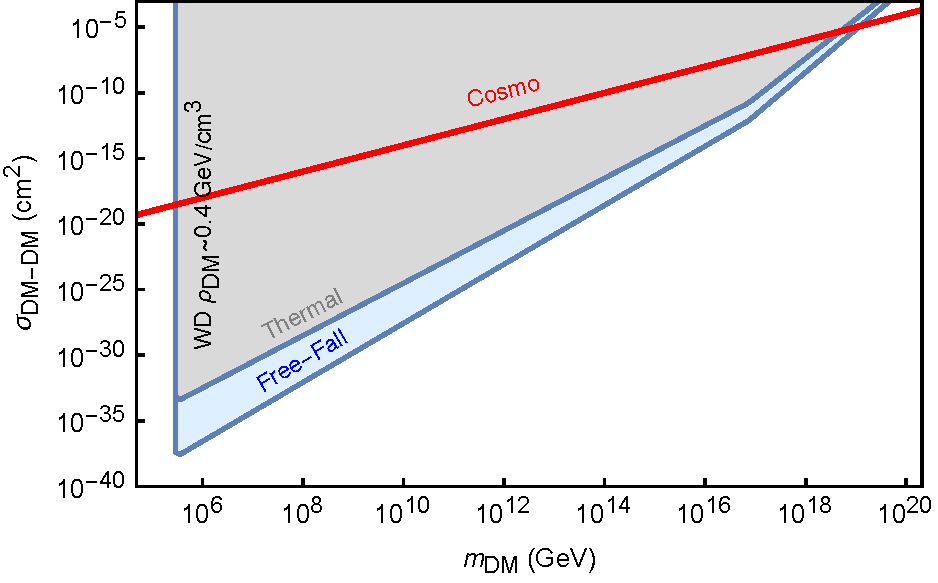
\includegraphics[scale=.35]{multicollision.pdf}
\caption{Constraints on DM-DM annihilation cross-section into SM particles which deposit their energy compactly within a trigger size $\lambda_T$ during self-gravitational collapse in a WD. Bounds come from observation of a single $1.25~M_{\astrosun}$ WD assuming efficient capture of the DM ($\Gamma_\text{cap} \sim \Gamma_\text{trans}$). We also assume the DM collapse is stabilized by formation of a BH.}
\label{fig:multicapture}
\end{figure}
The bounds in Figure \ref{fig:multicapture} are valid for any SM annihilation products which deposit their energy compactly upon release within a trigger size $\lambda_T$.
The plotted region is the set of all paramteres which satisfy \eqref{eq:collapsecondition} and \eqref{eq:multcolboom}----with $N_\text{multi}$ given by \eqref{eq:nmulti}---assuming that the DM collapse is stabilized by formation of a BH. 
One can check that the additional conditions \eqref{eq:steadycollect} and \eqref{eq:xicondition} are also satisfied for such parameters. 
We can qualitatively understand the range of excluded cross sections as follows:
If $\sigma_{\chi \chi}$ is too large, then the DM will effectively deplete before reaching the critical number needed for collapse.
However, $\sigma_{\chi \chi}$ cannot be arbitrarily small while still satisfying the boom condition \eqref{eq:multcolboom}. 

Of course, the constraints on multiple DM collisions in a collapse can be made concrete for a specified DM interaction. 
As in Section \ref{sec:previous}, we consider the case where the DM is captured in a WD via elastic scatters. 
Suppose the DM scatters off nuclear targets through Z boson exchange, with a per-nucleon cross section
\begin{equation}
\label{eq:Zscattering}
\sigma_{\chi n} \sim \frac{G_F^2 \mu_{\chi n}^2}{2\pi} Y^2 \left [\frac{(A-Z) - (1-4 \sin^2{\theta_W})Z}{A} \right ]^2 \approx 10^{-39} ~\cm^2,
\end{equation}
where $G_F$ is Fermi's constant and $Y$ is the hyper-charge of the DM. 
In order to satisfy the XENON bound \eqref{eq:xenon}, such a DM must be sufficiently heavy $m_\chi \gtrsim 10^9 ~\GeV$. 
In addition, suppose such a DM has an annihilation cross section into electroweak gauge bosons.
This is of course a generic class of DM models, although there are many specific manifestations of these interactions, e.g. heavy sneutrino DM. 
A particular example considered by \textcolor{blue}{keisuke and friends} is a type of heavy WIMPzilla DM they call ``GUTzilla".
The naive estimate for such an annihilation cross section is of order
\begin{equation}
\sigma_{\chi \chi} v \sim \frac{1}{8\pi} \frac{g_W^2}{m_\chi^2}.
\end{equation}
However, the cross section can be larger, e.g. due to a Sommerfeld enhancement. 
There is also the possibility of an upper limit on the annihilation cross section (the so-called unitarity limit) if the DM is ``point-like" in nature:
\begin{equation}
\sigma_{\chi \chi} v \lesssim \frac{4 \pi}{m_\chi^2} \frac{1}{v}.
\end{equation}
W and Z bosons decay predominantly to quarks with a decay length of order
\begin{equation}
\delta_W \sim \frac{8\pi}{g_W^2 m_W} \l \frac{m_\chi}{m_W} \r \sim 10^{-7} ~\cm \l \frac{m_\chi}{10^{9} ~\GeV} \r. 
\end{equation}
Since hadrons stop efficiently within the trigger size at all energies and WD densities \textcolor{blue}{elaborate}, the heating length of any one annihilation is set by the decay length of the gauge boson. 
Evidently, DM masses $m_\chi > 10^{11}$ will have a heating length larger than the trigger size of a $1.25~M_{\astrosun}$ WD.
In this case we take $L_\text{heat} = L_0 \approx \delta_W$ and, as expected, the boom condition on the DM becomes more stringent as more collisions are needed to deposit sufficient energy in the larger volume $L_0^3$ to trigger a SN. 
\begin{figure}
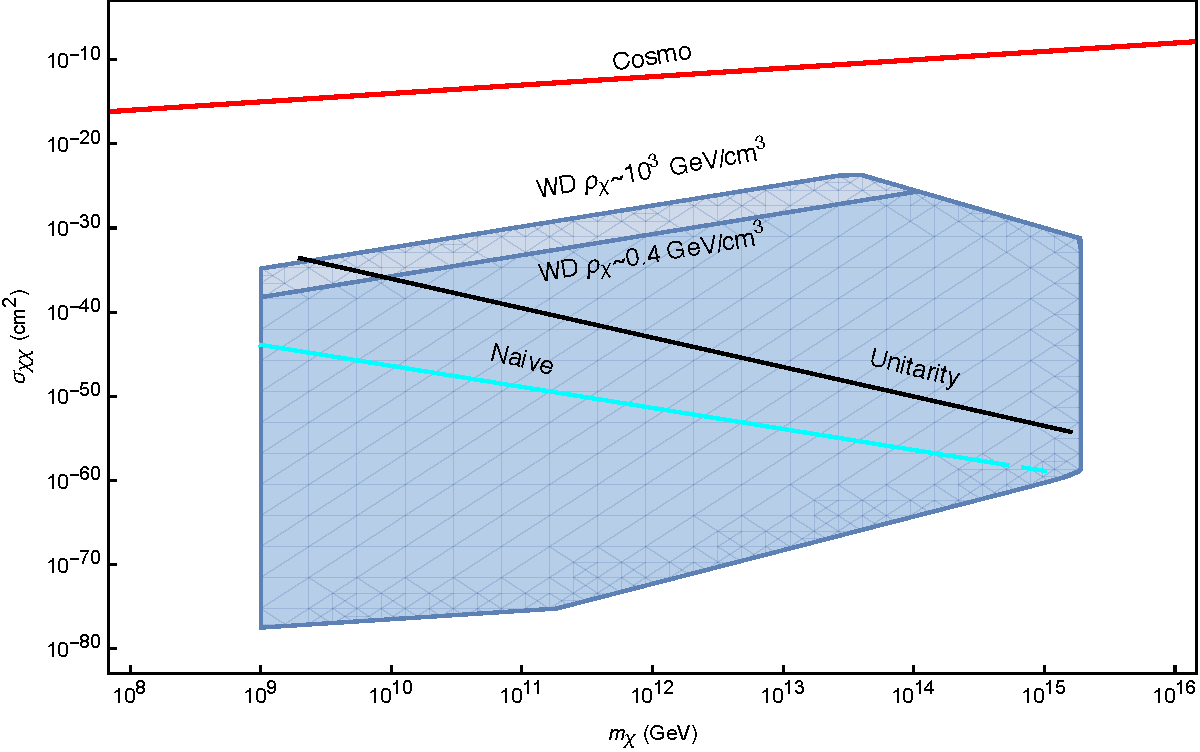
\includegraphics[scale=.35]{GZcapture.pdf}
\caption{Constraints on a generic class of DM models which elastically scatter off nuclei through Z boson-exchange and annihilate into electroweak gauge bosons. Bounds come from observation of a single $1.25~M_{\astrosun}$ WD.
We assume the DM collapse is stabilized by formation of a BH. Also shown are the naive order of magnitude (blue) estimate and unitarity limit (black) for this annihilation cross section.}
\label{fig:multicapture}
\end{figure}

\end{document}